\chapter{Integración}\label{chap:Integration}
Trazado el esquema del trabajo a realizar, el siguiente es lógicamente llevarlo a cabo. Las soluciones empleadas para todo el proceso será lo que componga este capítulo.

\section{Desarrollo de la API}
Si bien en la sección~\ref{sec:dis_api} ya se habló de la estructura con la que nuestra API contaría, en esta ocasión se contará con todo detalle el modo en el que esta ha sido desarrollada. Se describirán los puntos más importantes de cada una de las clases así como el modo en que fueron originados. Naturalmente, no se pretende explicar todo el contenido, pues no es su propósito. Se evitará así explicar en muchos casos métodos y propiedades privadas para centrarnos en aquellas públicas.

Para finalizar se explicará la relación existente entre las clases con ayuda de un diagrama UML así como la forma en la que estas han sido compiladas para ser unificadas como librería.

Todas estas clases conforman un único \texttt{namespace} o espacio de nombres. Conviene recalcar que la API ha sido enteramente desarrollada desde cero.

\subsection[GNS3sharp]{\href{https://github.com/aorestr/GNS3sharp/blob/master/gsn3sharp.cs}{GNS3sharp}}
\subsubsection{Constructor}
El constructor de \GNSCS~es sin duda uno de los elementos más importantes de toda a API. ¿Por qué? Tendrá la responsabilidad de conectarse al servidor de GNS3, recibir todos los datos de un cierto proyecto que solicitemos, procesarlos y guardarlos de tal forma que sean útiles. Su cabecera se muestra justo a continuación:
\begin{lstlisting}[language={[Sharp]C}, caption={Cabecera del constructor de \texttt{GNS3sharp}}, label={gnscs1}]
public GNS3sharp(string _projectID, string _host = "localhost", ushort _port = 3080)
\end{lstlisting}

Cosas que serán necesarias entonces para inicializarlo:
\begin{itemize}
\item \textbf{ID del proyecto}: cada proyecto de GNS3 tiene un ID asociado que el servidor guarda junto a su referencia. Más adelante, en la subsección \ref{subsec:aux}, veremos cómo no es necesario conocer el ID del proyecto sino que con el nombre del mismo será más que suficiente.
\item \textbf{Host}: la dirección del equipo donde el servidor está alojado. Por defecto se toma \texttt{localhost}; se supone que la mayor parte de las veces se encontrará en el mismo equipo desde el que se utiliza la API.
\item \textbf{Puerto}: además de la dirección del servidor, es necesario conocer el puerto en el que está montado. GNS3 determina el \texttt{3080} por defecto.
\end{itemize}

De acuerdo, ¿y qué hace exactamente con estos tres parámetros?
\begin{enumerate}
\item Crea la cadena de texto de la URI donde está el recurso asociado a los nodos del proyecto. En esta dirección existe únicamente un JSON con toda la información sobre él. Se instancia un cliente web y \textbf{se descarga el recurso como cadena de texto}.

\item Hay que \textbf{deserializar el JSON}. Este paso no es en absoluto trivial, ya que los métodos de \textit{Json.NET} son incapaces de extraer los datos que necesitamos directamente. Así que, valiéndonos de las herramientas en forma de clases que nos ofrece, lo hacemos manualmente.
\begin{lstlisting}[language={[Sharp]C}, caption={Deserialización de JSON}, label={gnscs2}]
// JSON array object
JArray jsonArray = JArray.Parse(json);
Dictionary<string,object> tempDict = new Dictionary<string, object>();

// Variables in which store the JSON info temporaly
string name; object value;        
if (jsonArray.HasValues){
    foreach (JObject jO in jsonArray.Children<JObject>()) {
        foreach (JProperty jP in jO.Properties()) {                
            name = jP.Name;
            value = (object)jP.Value;
            tempDict.Add(name,value);
            // The last key of every node
            if (jP.Name.Equals(lastKey)) {
                // If we do not copy the content of the dictionary into another
                // we will be copying by reference and erase the content once
                // we 'clear' the dict
                Dictionary<string, object> copyDict = new Dictionary<string, object>(tempDict);
                dictList.Add(copyDict);
                tempDict.Clear();
            }
        }
    }
}
\end{lstlisting}
Sin entrar mucho al detalle, lo que hace es parsear el objeto como objeto de tipo \texttt{JArray} y luego este se discretiza por cada elemento de esa cadena. Cada elemento representa a un nodo. Se recorre a su vez cada subelemento que lo conforma, que no son más que sus pares \textit{llave-valor}.

Los datos que se han extraído se guardan en una lista de diccionarios de par \texttt{<string,object>}. Se usa la clase genérica \texttt{object} porque el tipo del valor asociado a la clave varía.

\item Se hace lo mismo para los enlaces. El proceso es similar.

\item A partir de los objectos extraídos de la deserialización del JSON, se \textbf{crean las instancias representantes} de los nodos del proyecto. Existe un problema de cierta gravedad en esto: en el JSON no existe ningún parámetro que explicite de que tipo de nodo estamos hablando. Es decir, que no podemos conocer directamente con qué aparato concreto estamos tratando.

La solución que nosotros hemos tomado para sortear este problema es el añadir una etiqueta al nombre del nodo en el momento de la creación de la red en GNS3. Por ejemplo, si el nodo es un \textit{VPC} (nodo predefinido y propio del simulador), su nombre sería de la forma ``[VPC]NombreDelNodo''. Será necesario entonces definir una etiqueta por cada tipo de aparato a utilizar.

Sin embargo, sigue existiendo un problema de peso en todo esto: no conocemos el tipo de cada nodo antes del tiempo de ejecución (\textit{runtime}, en inglés) del código. En otras palabras, hasta el momento de la descarga y el análisis del JSON es imposible saber con qué tipo de nodos estamos lidiando, con lo que es a su vez imposible escribir el constructor que se va a utilizar. Recordemos que nuestra intención es usar una clase por cada modelo de nodo concreto. Por supuesto, se podría crear una sentencia condicional en la que, dependiendo de la etiqueta, llevara al constructor de una clase u otra. Sin embargo, requeriría de muchas líneas de código y sería necesario añadir más cada vez que se introduzca una nueva clase de modelo de aparato en la API.

La solución pasa entonces por lo que en programación se conoce como \textit{reflexión}. Poniéndolo en términos puramente técnicos: ``inspeccionar los metadatos y el código compilado en tiempo de ejecución se llama reflexión''\cite{csnutshell}.

\begin{lstlisting}[language={[Sharp]C}, caption={Instanciación de los nodos}, label={gnscs3}]
System.Reflection.ConstructorInfo ctor; int i = 0;
try{
    foreach(Dictionary<string, object> node in JSON){
        try{
            Console.WriteLine($"Gathering information for node #{i}... ");

            // Get the main constructor of the node type
            ctor = Aux.NodeType(node["name"].ToString()).GetConstructors(
                System.Reflection.BindingFlags.NonPublic | System.Reflection.BindingFlags.Instance
            ).Last();

            // Invoke the previous constructor and create the instance through it
            listOfNodes[i] = (Node)ctor.Invoke(
                new object[]{
                    node["console_host"].ToString(), 
                    ushort.Parse(node["console"].ToString()), 
                    node["name"].ToString(),
                    node["node_id"].ToString(),
                    GetNodeListOfPorts(node)
                }
            );
            
            nodesByName.Add(listOfNodes[i].Name, listOfNodes[i]);
            nodesByID.Add(listOfNodes[i].ID, listOfNodes[i]);
        } catch(Exception err1){
            Console.Error.WriteLine(
                "Impossible to save the configuration for the node #{0}: {1}", 
                i.ToString(), err1.Message
            );
        }
        i++;
    }
} catch(Exception err2){
    Console.Error.WriteLine(
        "Some problem occured while saving the nodes information: {0}",
        err2.Message
    );
    listOfNodes = null;
}
\end{lstlisting}
Con esto en mente pues, tomamos el tipo de la clase asociada al aparato mediante la etiqueta que ya hemos mencionado. Obtenemos gracias a él el constructor que nos es útil. El siguiente paso es invocarlo para generar la instancia del objeto. Previamente se pensó en utilizar el método \texttt{Activator.CreateInstance()}, que instancia un objeto directamente con los metadatos del tipo representante (representados a su vez por la clase \texttt{System.Type}) y los parámetros del constructor, pero solo funciona cuando los constructores son públicos y no es el caso de aquellos que usamos.

Añadimos la instancia a una lista donde se guardan todos los objetos representantes de los nodos. Esta propiedad se verá más adelante.

La obtención de las interfaces que cada nodo posee así como de cuáles están libres y cuáles están usadas por cierto enlace requiere de más trabajo que no se considera necesario explicar aquí.

\item Es ahora el momento de instanciar los enlaces a través de la información extraída previamente. Aunque el problema que vimos con los nodos no se va a dar aquí, la obtención de los enlaces y sus parámetros tampoco es fácil. La principal dificultad aparece, una vez más, cuando se trata con las interfaces de los nodos.

\begin{lstlisting}[language={[Sharp]C}, caption={Matcheo entre los enlaces y las interfaces de los nodos}, label={gnscs4}]
List<Dictionary<string,object>> dictList = null;
try{
    dictList = DeserializeJSONList(nodesJSON, "port_number");
} catch (Exception err){
    Console.Error.WriteLine(
        "Some problem occured while trying to gather information about the nodes connect to the link: {0}",
        err.Message
    );
}

if (dictList.Count > 0){
    // Iterates through the JSON dictionary
    foreach (Dictionary<string, object> nodeTemp in dictList){
        // Iterates through the nodes the link connects
        foreach (Node node in link.Nodes){
            if (node != null && node.ID.Equals(nodeTemp["node_id"].ToString())){
                // Search for the port that matches the found one
                var foundPort = node.Ports.Where(
                    x => (
                        x["adapterNumber"].ToString() == nodeTemp["adapter_number"].ToString() &&
                        x["portNumber"].ToString() == nodeTemp["port_number"].ToString()
                    )
                );
                // If exists, add the link into the key "link" of the ports list
                // of dictionaries of the node
                if (foundPort.Count() > 0) foundPort.First()["link"] = link;
            }
        }
    }
}
\end{lstlisting}

Una vez localizada la sección relacionada con los nodos en el diccionario que contiene la información de los enlaces extraída del JSON, se deserializa y se hace un barrido por entre esos nodos. Hecho esto, se busca entre los nodos que ya tenemos almacenados aquel que posea la misma ID que el del nodo sobre el que estamos barriendo. Si se encuentra, se busca la interfaz del mismo que dicte el nodo del barrido. De encontrarse, el puerto (usado aquí como sinónimo de interfaz) del nodo que teníamos almacenado guardará la información del enlace que contiene todos esos nodos que se están analizando. Es bastante confuso, sí.

El método principal que se encarga de la extracción de los enlaces, \texttt{GetLinks()}, se verá ayudado por un par de funciones declaradas localmente. Estas funciones locales aparecen por vez primera en C\#7.

Se guardan todos estos enlaces como lista en otra de las propiedades que se verán más adelante.

\item Finalmente, se añade a cada nodo la información de los enlaces a los que está conectado.

\end{enumerate}

\subsubsection{Propiedades}
\begin{itemize}
\item \texttt{ProjectID}, \texttt{Host} y \texttt{Port}: propiedades que se toman directamente de los parámetros que el constructor necesitaba.
\item \texttt{NodesJSON} y \texttt{LinksJSON}: diccionarios que contienen los JSON descargados desde el servidor una vez han sido parseados. Por lo general esta propiedad no tendría porque ser usada por un usuario que no esté desarrollando la API, pero se mantiene como \texttt{public} por si hay algún caso en el que sí.
\item \texttt{Nodes} y \texttt{Links}: posiblemente las propiedades más importantes de la clase. Son listas que contienen los objetos que representan los nodos y enlaces, respectivamente, del proyecto.
\end{itemize}

\subsubsection{Métodos}
La mayor parte de los métodos de esta clase son privados, pues son usados internamente como subrutinas de otros métodos más grandes. Sin embargo podemos encontrar algunos accesibles desde fuera de la clase:
\begin{itemize}
\item \texttt{StartNode()} y \texttt{StopNode()}: activan/desactivan un nodo del proyecto. Esto se consigue haciendo uso del método POST de REST hacia la URI correspondiente al nodo. En el código se lleva a cabo mediante la clase \texttt{System.Net.Http.HttpClient}, que provee las herramientas suficientes para enviar y recibir datos de un recurso web.

\begin{lstlisting}[language={[Sharp]C}, caption={Activación/desactivación de un nodo}, label={gnscs5}]
// First part of the URL
string URLHeader = $"http://{host}:{port}/v2/projects/{projectID}/nodes";

// Pack the content we will send
ByteArrayContent byteContent = null;
try{
    string content = JsonConvert.SerializeObject(new Dictionary<string, string> { { "", "" } });
    byteContent = new ByteArrayContent(System.Text.Encoding.UTF8.GetBytes(content));
    byteContent.Headers.ContentType = new MediaTypeHeaderValue("application/json");
} catch(JsonSerializationException err){
    Console.Error.WriteLine("Impossible to serialize the JSON to send it to the API: {0}", err.Message);
}

if (byteContent != null){
    try{
        responseStatus = HTTPclient.PostAsync(
            $"{URLHeader}/{node.ID}/{status}", byteContent
        ).Result.IsSuccessStatusCode;
    } catch(HttpRequestException err){
        Console.Error.WriteLine("Some problem occured with the HTTP connection: {0}", err.Message);
        responseStatus = false;
    } catch(Exception err){
        Console.Error.WriteLine("Impossible to {2} node {0}: {1}", node.Name, err.Message, status);
        responseStatus = false;
    }
} else{
    responseStatus = false;
}
\end{lstlisting}

\item \texttt{StartProject()} y \texttt{StopProject()}: activan/desactivan todos los nodos del proyecto. Se intentó paralelizar el activado/desactivado de los nodos sin resultado.
\item \texttt{SetLink()}: pasándole los objetos representantes de dos nodos del proyecto, es capaz de descubrir cuáles de sus interfaces están vacías y, de haber, crea un enlace entre ellas. También se consigue mediante POST. Actualiza \texttt{Links} y otra serie de parámetros tras la inserción. Es un método de cierta longitud (algo más de 100 líneas sin contar otras definidas fuera de las que hace uso). En este método y en similares es muy recurrido el tipo \texttt{dynamic}, que obliga al compilador a averiguar el tipo real de la variable en el momento de ejecución del código. Algo similar a lo que ocurre en lenguajes interpretados como Python y Matlab.
\item \texttt{EditLink()}: método polimórfico, pues dependiendo de si su parámetro es un \LINK~o dos \NODE~su comportamiento varía. Se parece a \texttt{SetLink()} pero este hace PUT y no POST a la URI. Ambas formas del método llaman a un método interno de \LINK. Tal y como su nombre indica, edita un enlace, permitiendo hacer variar los parámetros del mismo.
\item \texttt{RemoveLink()}: con la misma base polimórfica que el anterior. Elimina un enlace del proyecto de GNS3 con un DELETE e inmediatamente a su representante objeto.
\item \texttt{GetNodeByName()} y \texttt{GetNodeByID()}: dado un nombre o un identificador, respectivamente, devuelve el objecto representante de tal nodo.
\end{itemize}

\subsection[Node]{\href{https://github.com/aorestr/GNS3sharp/blob/master/node.cs}{Node}}
\subsubsection{Constructor}
El constructor principal de \NODE~solo es llamado desde \GNSCS. Es bastante sencillo: asigna parámetros básicos que la instancia de \GNSCS~toma del servidor. Entre ellos se encuentra la dirección del nodo. Gracias a ella y mediante otro método interno de la clase, se crea un cliente TCP y se establece un flujo de conexión para el envío y recepción de mensajes.

\begin{lstlisting}[language={[Sharp]C}, caption={Establecimiento de la conexión con el nodo}, label={node2}]
protected (TcpClient Connection, NetworkStream Stream) Connect(int timeout = 10000){
    // Network endpoint as an IP address and a port number
    IPEndPoint address = new IPEndPoint(IPAddress.Parse(this.consoleHost),this.port);
    // Set the socket for the connection
    TcpClient newConnection = new TcpClient();
    // Stream used to send and receive data
    NetworkStream newStream = null;
    try{
        newConnection.Connect(address);
        newStream = newConnection.GetStream();
        newStream.ReadTimeout = timeout; newStream.WriteTimeout = timeout;
    } catch(Exception err){
        Console.Error.WriteLine("Impossible to connect to the node {0}: {1}", this.name, err.Message);
        newConnection = null;
    }
    return (newConnection, newStream);
}
\end{lstlisting}

Especial atención a este método, que devuelve una tupla (recordemos, también nuevo en C\#7) en lugar de una simple variable.

Para que solo clases que pertenecen a esta librería puedan hacer uso del constructor, se ha aplicado el modificador de clase \texttt{internal}, el cual solo permite llamadas desde el espacio de nombres donde esté definido. Encapsulamiento en estado puro. La API no permite la creación de nodos nuevos así que se ha optado por ocultar este método del desarrollador final.

No obstante, sí que se incluye un constructor-clonador. Se trata de un constructor de clase cuyo parámetro de entrada es otro \NODE, de forma que se replica enteramente en una nueva instancia.

\begin{lstlisting}[language={[Sharp]C}, caption={Clonador de nodos}, label={node2}]
public Node(Node clone){
    this.consoleHost = clone.ConsoleHost; this.port = clone.Port;
    this.name = clone.Name; this.id = clone.ID; this.ports = clone.Ports;
    this.tcpConnection = clone.TCPConnection; this.netStream = clone.NetStream;
}
\end{lstlisting}

\subsubsection{Propiedades}
\begin{itemize}
\item \texttt{ConsoleHost} y \texttt{Port}: dirección y puerto donde el nodo está ubicado. Gracias a estos datos podremos establecer una conexión con el aparato.
\item \texttt{Name} y \texttt{ID}: nombre e identificador único del nodo. El nombre debería comenzar por \textit{[$<$EtiquetaDelNodo$>$]} para que \GNSCS~sea capaz de construir el objeto con la clase asociada a tal aparato.
\item \texttt{Ports}: interfaces que posee el nodo. Es un diccionario de tres llaves: ``adapterNumber'', ``portNumber'' y ``link''. Los dos primeros son parámetros que GNS3 asigna a las interfaces. El último guarda la referencia del enlace asociado a la interfaz en caso de que esté siendo utilizada y \texttt{null} si no.
\item \texttt{LinksAttached}: lista de \LINK. Referencias a los que el nodo está conectado.
\end{itemize}

\subsubsection{Métodos}
Esta clase destaca por sus dos métodos principales: \texttt{Send()} y \texttt{Receive()}.

\begin{itemize}
\item \texttt{Send()}: haciendo uso del flujo establecido durante la creación del objeto, se envía una cadena de texto previamente convertida a bytes. Antes de enviar cualquier mensaje, comprueba que es posible escribir en el canal.

\begin{lstlisting}[language={[Sharp]C}, caption={Envío de mensajes a un nodo}, label={node3}]
byte[] out_txt = Encoding.Default.GetBytes($"{message}\n");
this.netStream.Write(buffer: out_txt, offset: 0, size: out_txt.Length);
this.netStream.Flush();
\end{lstlisting}

\item \texttt{Receive()}: algo más complejo que \texttt{Send()}, hace también uso del canal establecido, aunque necesita de pasos adicionales para gestionar correctamente la información que se recibe.

Cada mensaje recibido se convierte en una cadena de texto que va siendo añadida a una lista. A cada nueva recepción se consulta al canal si existe nueva información a leer; si no, se esperan unos segundos confiando en que existan datos a procesar por parte del servidor. Se vuelve a hacer la comprobación y, si efectivamente no queda nada más por leer, se analizan las líneas recibidas en busca de caracteres inválidos y se guardan. 

\end{itemize}

\subsubsection{Destructor}
Esta es la única clase de la librería que hace uso de un destructor personalizado. Los destructores ayudan a definir las sentencias que serán ejecutadas junto antes de que el objeto en cuestión sea destruido (se desreferencie).

Únicamente se encarga de cerrar la conexión establecida con el nodo.

\subsection{Herederos de Node}
La clase \NODE~no hace más que de padre para todo un abanico de clases. A partir de ahí se crea una estructura en árbol desde la que se ramifica una serie de subclases. Las tres herederas directas son \texttt{Router}, \texttt{Switch} y \texttt{Guest}, correspondientes a los tres amplios grupos de nodos que pueden encontrarse en GNS3. Estas tres clases son abstractas; su labor no es otra que la de declarar métodos importantes que cada uno de estos aparatos se espera que posean.

La definición de los métodos se encuentra en sus clases herederas, que no representan otra cosa que dispositivos concretos. Pongamos un ejemplo para que se vea más sencillo:

\NODE~es la clase padre. Define el constructor, la forma de establecer la conexión con los nodos y los métodos para enviar y recibir mensajes de estos. De esta clase parte otra, \texttt{Router}, que por consiguiente es hija suya. Esta clase declara métodos abstractos que se espera que las clases representantes de los routers posean, como por ejemplo \texttt{GetIPByInterface()}, que dado el nombre de una interfaz ha de ser capaz de averiguar cuál es su IPv4 asociada. Finalmente, la clase \texttt{OpenWRT} va a heredar de \texttt{Router}. Definirá los métodos abstractos de la anterior y los suyos propios.

Es muy importante señalar que cada una de estas clases representantes de aparatos concretos deberán contar con una propiedad estática que contiene la etiqueta que el nodo deberá tener en su nombre. De nuevo con ejemplo: si queremos que el constructor de \GNSCS~pueda construir correctamente el objeto representante a un router OpenWRT de nuestro proyecto de GNS3, es necesario que a este se le ponga por nombre algo como \textit{[OPENWRT]NombreDelRouter}. De esta forma, automáticamente y una vez más haciendo uso de reflexión, la API es capaz de encontrar la clase a la que se hace referencia.

\begin{lstlisting}[language={[Sharp]C}, caption={Etiqueta de \texttt{OpenWRT}}, label={herederosnode1}]
private const string label = "OPENWRT";
/// <summary>
/// Label you must set in the name of the node at the GNS3 project
/// <para>Name of the node must look like "[OPENWRT]Name"</para>
/// </summary>
/// <value>Label as a string</value>
public static string Label { get => label; }
\end{lstlisting}

Si se hace correctamente, se instanciará un objeto \texttt{OpenWRT}. De lo contrario, se optará por el genérico \NODE.

Este punto del trabajo es importante. Una de las cosas que más nos interesaban de la creación de la API era su reutilización por manos ajenas. La estructura establecida en ella permite que cualquiera que quiera hacer uso de ella y pretenda implementar un cierto tipo de nodos en su proyecto de GNS3 lo tenga fácil a la hora de crear un tipo que le dé soporte en la librería.

Actualmente GNS3 cuenta con implementaciones de docenas de dispositivos de gestión de red del mercado. Crear una clase representante de todas ellas es ciertamente un trabajo inviable. Sin embargo, se ha buscado que cada usuario que haga uso de ella lo tenga fácil para insertar la que necesite. Tan solo necesita añadir una clase que herede de su tipo de aparato correspondiente (\texttt{Router}...) y definir los métodos que le gustaría que esta tuviera.

El número de métodos definidos para cada clase va en función de las necesidades de cada uno. Un dispositivo real cuenta con cientos de funciones; abstraerlas todas como métodos es descabellado.

A continuación se muestra uno de los métodos que nosotros hemos generado para \texttt{OpenWRT}, clase que ha sido usada abundantemente en la integración final de este proyecto ya que el router al que hace referencia nos ha sido de gran utilidad.

\begin{lstlisting}[language={[Sharp]C}, caption={Método \texttt{GetIPByInterface()} de \texttt{OpenWRT}}, label={herederosnode2}]
public override string[] GetIPByInterface(string iface){

    string GetParameterIfconfig(string _iface, string type){

        string result = null; string command = null;
        if (type.Equals("IP"))
            command = $"ifconfig {_iface} | grep 'inet addr' | cut -d: -f2 | awk '{{print $1}}'";
        else if (type.Equals("NETMASK"))
            command = $"ifconfig {_iface} | grep 'inet addr' | cut -d: -f4 | awk '{{print $1}}'";
        if (command != null){
            string lineTemp;
            Send(command);
            foreach (string line in Receive()) {
                lineTemp = line.Trim();
                if (Aux.IsIP(lineTemp)){
                    result = lineTemp;
                    break;
                }
            }
        }
        return result;

    }

    return new string[]{ 
        GetParameterIfconfig(iface, "IP"), GetParameterIfconfig(iface, "NETMASK") 
    };
    
}
\end{lstlisting}

El método se encarga de encontrar la IP relacionada con cierta interfaz del router. Básicamente, envía un comando al router mediante \texttt{Send()} y de la respuesta obtenida con \texttt{Receive()} extrae la IP.

La conclusión que ha de sacarse de esto es que todos los métodos, o la mayor parte de ellos, van a ser definidos en base a estas dos funciones, \texttt{Send()} y \texttt{Receive()}. Podemos llevar esta lógica algo más allá: si no existe método creado en cierta clase para realizar una operación que nos es necesaria, podemos hacer uso de aquellas dos funciones para, sobre la marcha, conseguir lo que esperamos.

\subsection[Link]{\href{https://github.com/aorestr/GNS3sharp/blob/master/link.cs}{Link}}
\subsubsection{Constructor}
Una vez más, el constructor es únicamente accesible desde el espacio de nombres y solo será llamado desde \GNSCS. Se han definido dos concretamente: uno que supone que todos los parámetros del enlace de GNS3 son nulos (es un enlace ideal) y otro que supone que al menos uno de ellos es distinto.

\subsubsection{Propiedades}
\begin{itemize}
\item \texttt{ID}: identificador único del nodo. Como el resto de IDs, lo asigna automáticamente GNS3.
\item \texttt{Nodes}: array de objetos \NODE~que contienen los objetos representantes de los nodos que el enlace une en el proyecto.
\item Parámetros del enlace: \texttt{FrequencyDrop}, \texttt{PacketLoss}, \texttt{Latency}, \texttt{Jitter} y \texttt{Corrupt}. Son parámetros que GNS3 permite para eliminar idealidades de las conexiones. Todos son números enteros.
\end{itemize}

\subsubsection{Métodos}
Esta clase solo cuenta con un método, \texttt{EditLink()}. Permite editar uno de los parámetros del enlace. Para ello, además de ser este alterado en el objeto, se modifica en el proyecto de GNS3 haciendo un PUT a la URI asociada al enlace. Ya se mencionó este método tratando uno de los de \GNSCS.

\subsection{Clases auxiliares}\label{subsec:aux}
\begin{itemize}
\item \texttt{Aux}: define métodos de ayuda para otras clases del espacio de nombres como un identificador de direcciones IP. También se encarga de generar, mediante reflexión, un mapeo entre los tipos de nodos existentes en la API y la etiqueta asociada a ellos. Todo esto es realizado de forma automática.
\item \texttt{RoutingTable}: define una estructura para las tablas de enrutamiento. Es usada por las clases herederas de \texttt{Router} para una gestión más eficiente de esas tablas. Dentro de la propia clase se define un \texttt{struct} usado para trabajar más cómodamente con cada una de las rutas de la tabla. 
\item \texttt{ServerProjects}: en esta clase deben definirse métodos asociados a la URI del server donde se lista el conjunto de proyectos definidos en él. Por el momento solo cuenta con un método (\texttt{GetProjectIDByName()}) que extrae el ID de un proyecto dado su nombre, realmente útil a la hora de instanciar \GNSCS.
\end{itemize}

\subsection{Estructura de la API}
A continuación se muestra el diagrama UML de la API, desde el que puede observarse esquemáticamente el diseño de cada una de las clases y la relación que existe entre ellas.

\begin{figure}[h]
  \centering
  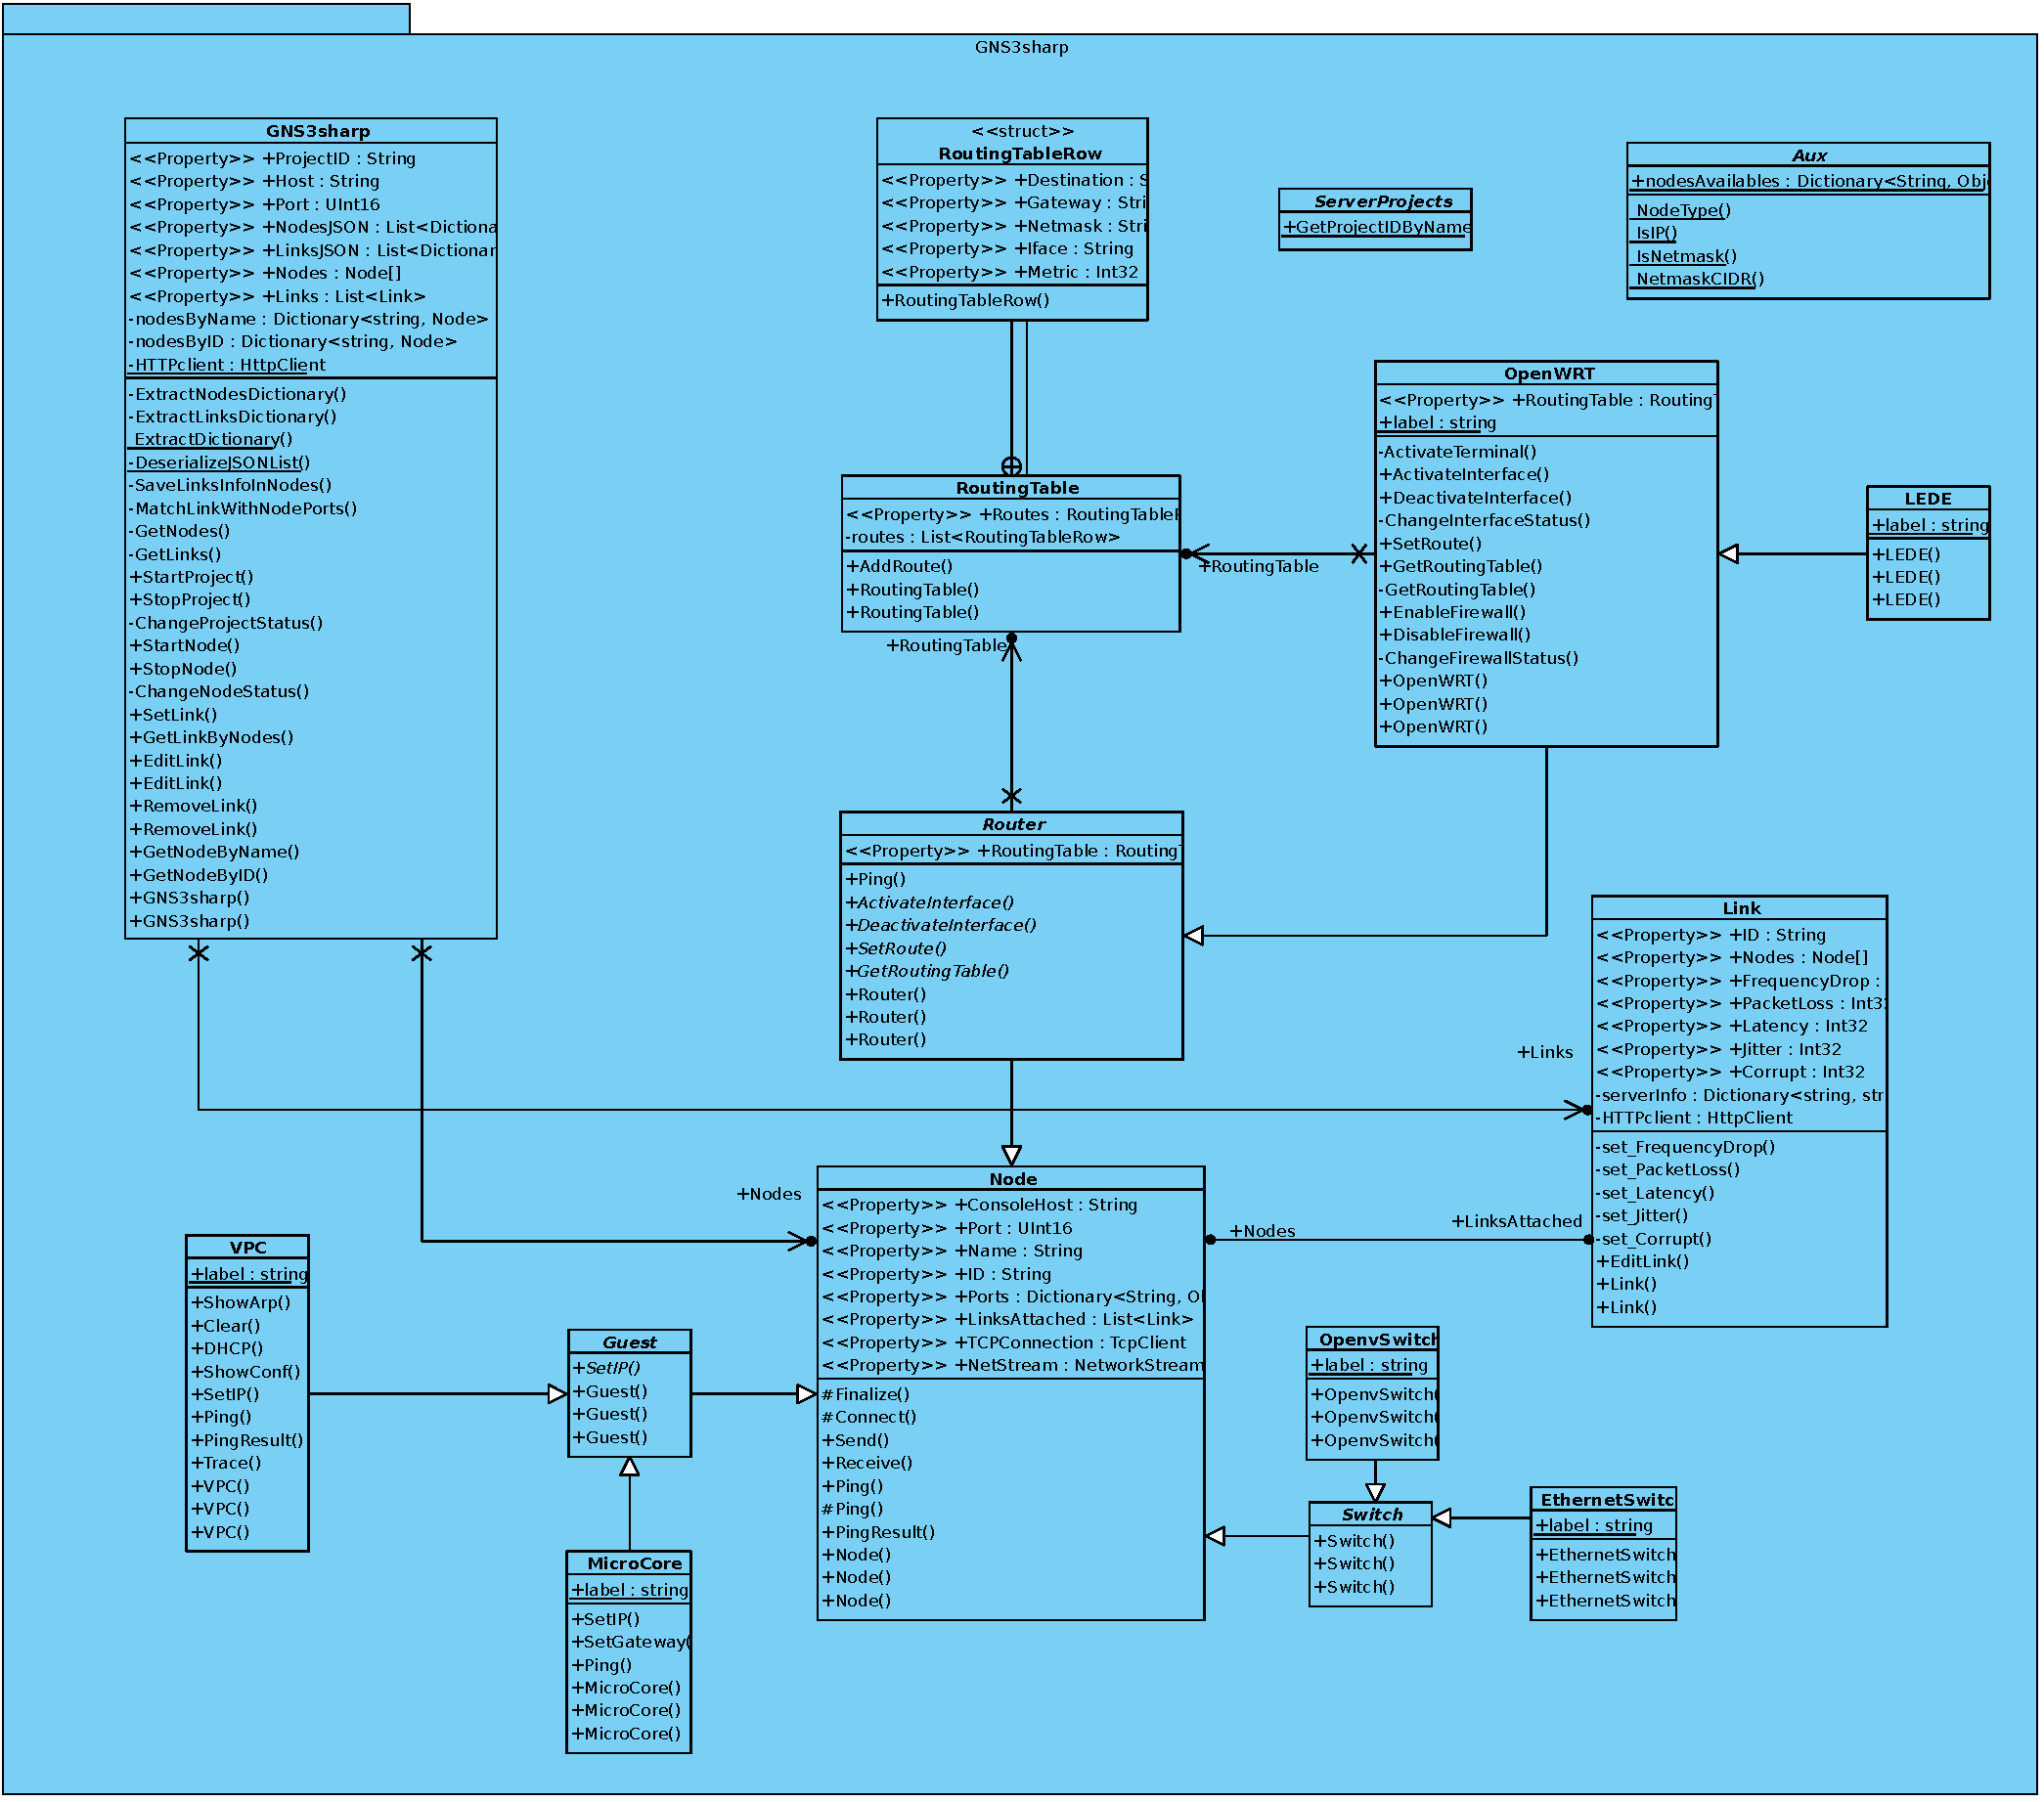
\includegraphics[scale=0.4]{imagenes/diagrama_api2}
  \caption{Diagrama UML de la API}
  \label{fig:uml_api}
\end{figure}

\subsection{Compilación}
C\# es un ``lenguaje gestionado'' (del inglés \textit{managed code}) pues es compilado en código gestionado. Este código gestionado es representado en un lenguaje intermedio. Aparece entonces la figura del \textit{Common Language Runtime} (CLR), núcleo del Microsoft .NET Framework. Se encarga de traducir este código intermedio al código nativo de la máquina desde la que se ejecuta.

Los contenedores de código gestionado se llaman ensamblados, y pueden ser archivos ejecutables (\textit{.exe}) o bien librerías (\textit{.dll})\cite{csnutshell}. Nuestro propósito es el de contener el código de la API en un ensamblado para librerías.

El editor de código Visual Studio de Microsoft tiene integradas decenas de herramientas para trabajar con proyectos dirigidos a .NET. Así, entre otras muchas cosas, facilita la compilación del código en C\# para extraer de él un ensamblado que pueda ser incluido en otro proyecto como librería externa.

\begin{figure}[h]
  \centering
  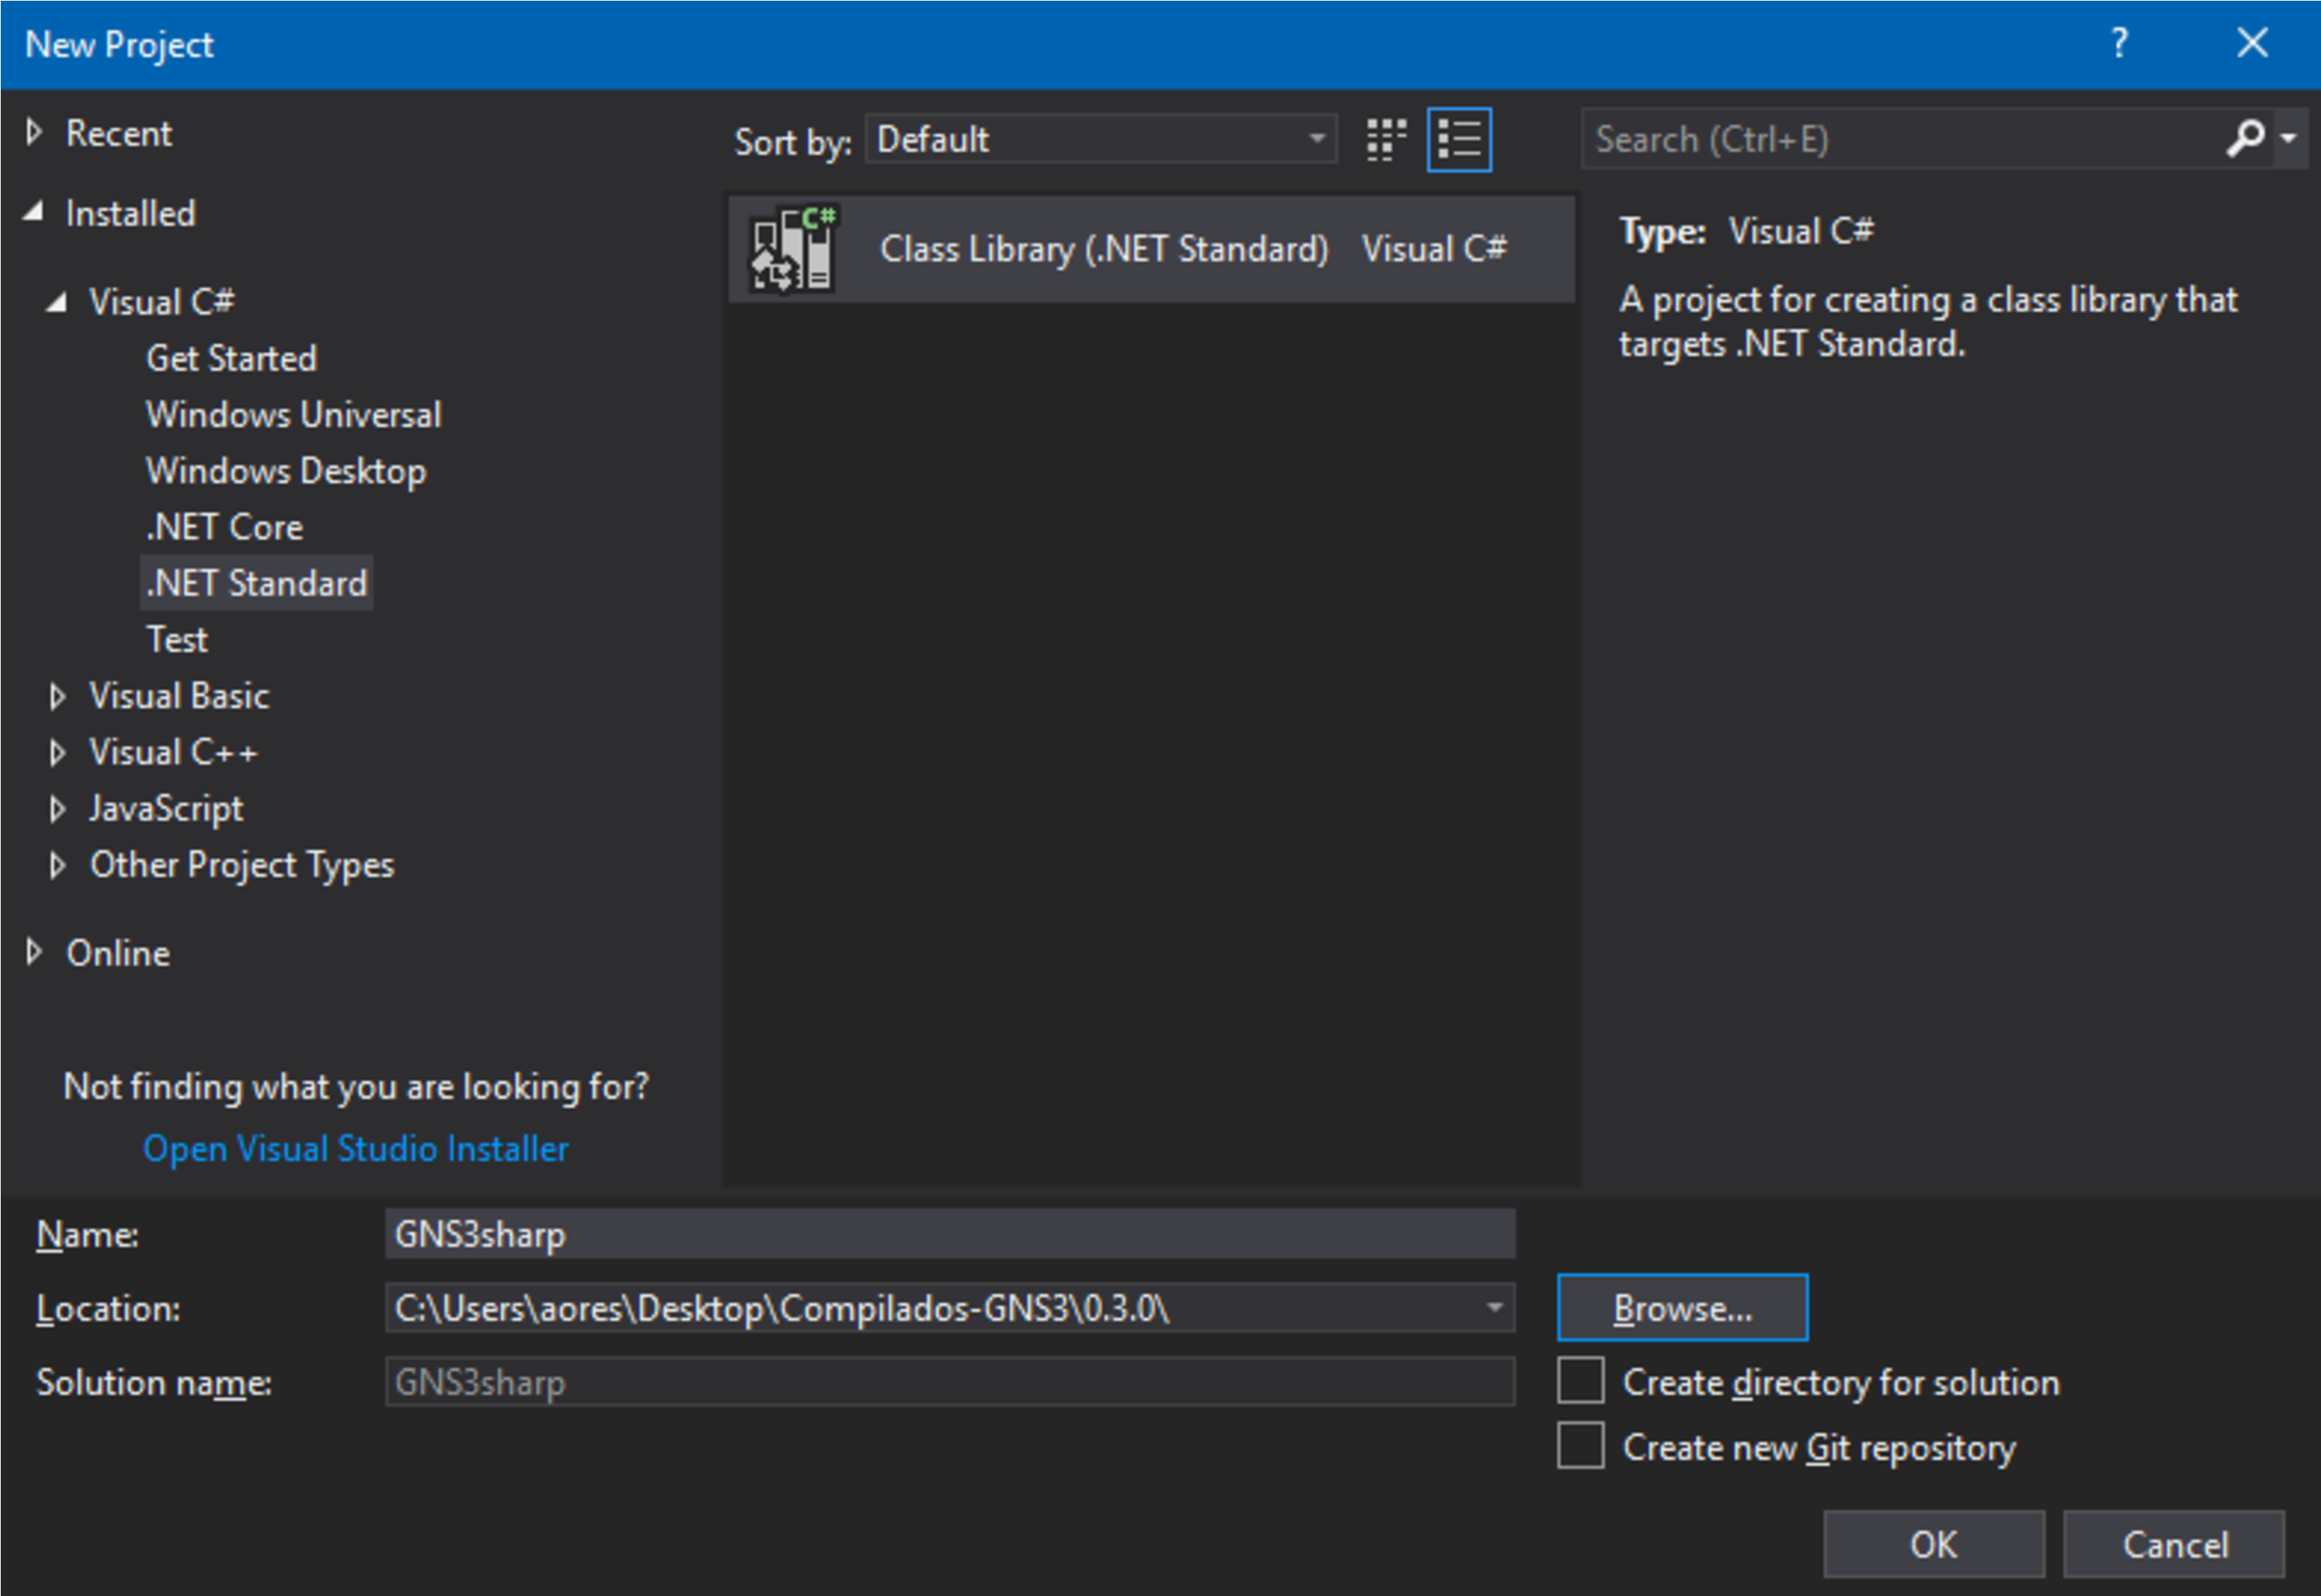
\includegraphics[scale=0.225]{imagenes/creacion_ensamblado}
  \caption{Elección del tipo de proyecto en Visual Studio 2017}
  \label{fig:creacion_ensamblado}
\end{figure}

Como framework con el que realizar la compilación se ha elegido \textit{.NET Standard 2.0}. De esta forma la librería será portable y correrá sin modificaciones en versiones modernas de todos los frameworks principales de .NET (.NET Core, .NET Framework...) pues únicamente posee el núcleo común de todos ellos. En realidad, .NET Standard no es un Framework: es simplemente una especificación que describe una base mínima de funcionalidad (tipos y miembros), que garantiza la compatibilidad con un cierto conjunto de frameworks.

Para el correcto ensamblado del código de la API hará falta la importación de dos librerías externas: \href{https://www.nuget.org/packages/Newtonsoft.Json/}{\textit{Json.NET}}, como ya se ha dicho en varias ocasiones, y \href{https://www.nuget.org/packages/Microsoft.CSharp/}{\textit{Microsoft.CSharp}}. Esta última, no incluida por defecto en .NET Standard, añade funcionalidades para la compilación dinámica de código (el modificador de acceso \texttt{dynamic} o el propio instanciador de clases por reflexión).

Con el fin de facilitar a los desarrolladores la importación de código de terceros, Visual Studio integra una herramienta que permite instalar esas dependencias en tus proyectos a través de \textit{NuGet}. NuGet es el formato de empaquetamiento de librerías de .NET para simplificar su compartición. Cuenta con una plataforma de hosting donde hospedar paquetes públicos paraser descrgados con facilidad por el resto de desarrolladores. La herramienta de Visual Studio se conecta directamente a este host, descarga el paquete y lo instala en el proyecto que esté siendo usado. Las dos librerías señaladas anteriormente se encuentran en tal plataforma.

Establecidos una serie de parámetros que servirán de metadatos para el ensamblado, se compila el proyecto. Visual Studio crea entonces el archivo \textit{.dll} así como un archivo \textit{.xml} que, enlazado al ensamblado, aporta la documentación de nuestra librería. Para lograr esto último fue necesario la inclusión de etiquetas XML como encabezado de cada uno elemento de la API (clases, métodos, propiedades...) cuya sintaxis puede \href{https://docs.microsoft.com/en-us/dotnet/csharp/programming-guide/xmldoc/xml-documentation-comments}{consultarse online}. Similar al Javadoc de Java.

Ya tenemos preparada la librería para que Unity haga uso de ella.

\section{Desarrollo del videojuego}
En esta sección se detalla la construcción del videojuego. En primer lugar se habla del juego en sí, qué se ha creado y qué no y qué se puede esperar de él. Inmediatamente después se describe el entorno generado en GNS3 para ser usado por Unity para, más adelante, mostrar cómo y qué ha sido desarrollado mediante él.

\subsection{Descripción del juego}

\subsection{El proyecto de GNS3}


\subsubsection{Aparatos usados}

\subsubsection{Despliegue}

\subsection{El proyecto de Unity}

\subsubsection{Materiales}

\subsubsection{Creación del juego}
